\hypertarget{Fundamentals of Overlapped Sounds}{%
\chapter{Fundamentals of Overlapped Sounds}\label{cha:fundamentals}}

In this thesis the core part in focussed on \emph{analysis} and \emph{processing} of sound recordings of music and speech, commonly referred to as \emph{audio signals}.
In this chapter, I therefore introduce basic concepts of digital audio signals which are relevant to apprehend the remaining chapters.

\hypertarget{Audio Signals}{%
\section{Audio Signals}\label{sec:specifics-of-audio-signals}}

When a sound wave travels through a medium like air it can be captured using a microphone by measuring the local pressure deviation over time.
Such a signal ca be written as a function \(x(t)\) continuous in both, time \(t \in \sR\) and the amplitude \(x(t) \in \sR\).
An \emph{audio signal} can simply be introduced as a signal that is meant to be perceived by the human auditory system --- through our ears.
Therefore, one could observe specifics properties of audio signals, consistent to the limitations of the human hearing system, for example in dynamics/loudness as well as a limited signal bandwidth.
In fact, many other signals exist with similar characteristics such as signals from finance, geophysics, meteorology or medical data.
The result is that often audio research is inspired by applications of other fields of signal processing and vice versa.

\hypertarget{digital-representations-of-audio-signals}{%
\subsection{Digital Representations of Audio
Signals}\label{digital-representations-of-audio-signals}}

To conveniently store, analyze or process audio signals, as of today, digital representations are used to leverage the processing capabilities of modern computing devices.
A digital audio signal can be obtained from an analog signal using analog-to-digital/digital-to-analog converters (ADC/DAC) which can be found in almost any every-day device such as laptops and smartphones.
In short, this process includes two steps, First, the continuous time signal \(x(t)\) is converted to a discrete time series, so that one sample\footnote{Please note, that the use of the word \emph{sample} will have different meanings in the context of machine learning, where a sample is an instance of a full signal instead of a single time step.} \(x_n\) is \emph{sampled} with equidistant steps \(T\) and Second, the amplitude values are \emph{quantized} resulting in vector \(\vx \in \sZ\), represented as a one dimensional time series of amplitudes.
An important parameter in the process of digitization is the sample rate \(F_s = 1/T\) where \(T\) is the sampling period.
Often, \(F_s\) has a significant effect on the quality of audio signals.
And, it is the objective of a real world audio system to not introduce perceptible degradation in audio quality when a digital signal is reproduced over headphones or loudspeakers.
Due to the Nyquist-Shannon sampling theorem the sample rate needs to be at least twice the band width of the analogue signal.
Since the hearing range of normal listening humans is
20~\si{\hertz} - 20~\si{\kilo\hertz}~\cite{fastl90, moore89}, typically for audio signals, 
sample rates of 44100~\si{\hertz} are chosen to facilitate the full human hearing range.
However, for many applications, a lower sampling rate is sufficient, e.g. in speech communication where intelligibility often is more important than quality.
For further details we refer the reader to audio signal processing basics such as~Chapter 1 in~\cite{proakis96} or Chapter 2 in~\cite{Mueller15}.

\hypertarget{time-frequency-representation}{%
\subsection{Time-Frequency Representation}\label{sub:time-frequency-representation}}

Real world sounds such as speech and music have periodicities.
Therefore, sounds are analyzed in the frequency domain which also improves the computational efficiency of signal processing methods.
This is commonly achieved through the use of discrete Fourier transform (DFT) and its fast FFT implementation~\cite{cooley65}. 
For details, the reader is referred to~Chapter 4 of~\cite{proakis96}.
At the same time, spectral representations relates to our human auditory system~\cite{zwicker13, moore89} allowing us to process sounds the way we perceive them.
\par
The periodicity of real world sounds, as mentioned above, usually only holds for short durations of several milliseconds, often referred to as ``quasi-stationarity''.
Therefore, we analyze and process short-time spectra, computed in an overlapped fashion, resulting in a \emph{time-frequency} (TF) representation.
The short-time Fourier transform (STFT) is the most commonly used TF representation~\cite{mcaulay86}.
It encodes the time-varying spectra into a matrix \(\mX\) with frequencies \(k\) and time frames \(n\).
\par
When sounds are processed in the time-frequency domain, the transformation greatly benefits from being invertible to reconstruct a time domain signal.
STFT matrices \(\mX \in \sC^{n \times k \times c}\) are complex and include phase information.
However, analysis and processing is often focussed  on the \emph{magnitude} \(|\mX|\) or the \emph{spectrogram} \(|\mX|^2\).

\subsection{Fundamental Frequency and Harmonicity}
% TODO: add note pitch vs pitch discussion
% TODO: Add STFT plot from Cello Dataset, showing f0, overtones vibrato extend etc.
% \cite{stoeter15acm}, to be downloaded in \cite{oss}

Speech and music signals are often characterized by its periodicity.
And it is this property we perceive as \emph{pitched}.
\emph{Pitch} is defined by Klapuri~\cite{klapuri06book} as 

\begin{quote}
``a perceptual attribute which allows the ordering of sounds on a frequency-related scale extending from high to low.''
\end{quote}

It is important to note that \emph{pitch} is a subjective measure.
The objective equivalent is referred to as the \emph{fundamental frequency} (\(F_0\))\footnote{Pitch and $F_{0}$ are often used synonymously in audio research. Even though this is incorrect, I sometimes may refer to other work where pitch instead of $F_{0}$ is used.}.
\(F_{0}\) can defined as the lowest frequency/partial of an harmonic signal.
All frequencies together formed by the integer multiples of the fundamental frequency are named \textit{harmonics}~\cite{schenker54}.
When the fundamental frequency changes, the frequencies of these harmonics changes accordingly.
This results in the typical comb-like structure of harmonic signals when analyzed in the time-frequency domain.
% TODO: An example of a harmonic signal can be seen in Figure~\ref{fig:cello} that depicts a single played note from a violoncello.
\par
An estimate of the fundamental frequency of a signal is required in various applications of audio and speech signal processing.
Some scenarios are targeted to extract the fundamental frequency of the predominant source~\cite{salamon12} in a mixture of other sources.
In other applications, algorithms are used to extract fundamental frequencies of multiple sources simultaneously present in a signal~\cite{klapuri03}.
However, the most common scenario in many works is to extract the fundamental frequency of a monophonic and harmonic audio signal containing speech or music~\cite{talkin95, boersma02, decheveigne02, resch07, tidhar10, christensen07}.
For a a detailed overview into the research field of pitch and \(F_{0}\), the reader is referred to~\cite{klapuri06book}.

\subsection{Time-Variant Audio Signals}\label{sub:time-variant-audio-signals}

Audio signals are considered to be stationary or time-invariant when certain properties such as the amplitude or the fundamental frequency of the signal do not change over time.
A stationary sound can be modified to turn it into time-invariant sound. 
In signal processing this is referred to as modulations and is, in fact, of paramount importance as it has enabled technologies such as radio transmission~\cite{shannon48}.
Modulations can be defined as time-variant functions that modulate a target parameter of signal over time.
In the case of audio signals, often both, the modulating function (modulator) and the signal being modulated are are periodic.
Signal modulations are often created intentionally but also occur naturally in many real-world audio signals such as speech.
In the following, I will present typical audio modulation categories and their cause, underlining the importance of them.

\subsubsection*{Audio Signal Communication}

The transmission of an audio signal using a modulator/demodulator (modem) system may be one of the most important applications for audio modulations. 
The principle is used the broadcasting of radio using a high frequency carrier signal that is modulated by an audio signal to be transmitted, which is assumed to be of slower frequency than the carrier signal.
The modulator is targeted to vary the amplitude or the frequency of the carrier signal.
If we imagine a sinusoidal carrier signal $x(t) = \cos \omega_c t$, \emph{amplitude modulation} (AM) is applying by a modulation function $a(t)$ so that:

% We assume that we can separate overlapping partials of the sources based on differences in amplitude and/or frequency modulation, resulting in the following model for a signal with $P$ commonly modulated partials
% \begin{equation}
%   \begin{array}{l}
%    x(n) = \displaystyle \sum_{p=1}^{P} \Big[\big(1 + a(n)\big) \\
%    \hspace{3.5em}\displaystyle \cdot\sin \Big(2\pi f_{p,0}\big(n + \frac{1}{f_{1,0}} \sum_{m=m_0}^{n}{f(m)} \big) + \phi_{p,0} \Big)\Big] ,
%   \end{array}
% \end{equation}
% where effectively the amplitude modulation is $a(n)$ and the frequency modulation of the first partial is $f(n)$.

\begin{equation*}
    s_{AM}(t) = a(t) \cos \left( \omega_{c} t\right).    
\end{equation*}

In comparison to AM, Frequency modulation (FM) varies the frequency of the carrier, so that:

\begin{equation*}
    s_{FM}(t) = A e^{j\left(\omega_{0} t + m \sin \left(\omega_ { m } t \right)\right)}
\end{equation*}

where A is the amplitude, $\omega_0$ is the carrier frequency, $\omega_m(\theta)$ is the instantaneous modulation frequency, and $m$ is the modulation index $m = \frac{\Delta \omega_0} { \omega_{m} }$.

It is well known that the Fourier spectrum of $z_{FM}(t)$ is not simple to comprehend due to its non-linearity and it involves computations using the Bessel function.
For applications where the modulation frequencies are a lot smaller than the carrier frequency, the spectrum that is caused by frequency modulations is similar to those of amplitude modulations.
This is the reason why algorithms that aim to capture the amplitude modulation will also capture part of the frequency modulation as well.
The total bandwidth in this scenario is approximately $2\Delta \omega_0$, as found by Carson in~\cite{carson22}.\par
For the purpose of audio communication, the modulation frequency or rate is defined by the bandwidth of the audio signal to be transmitted.
Modulations in music or speech are much slower --- typically up to 10~\si{\hertz} (slow) or up to 100~\si{\hertz} (medium/fast).

\subsubsection*{Modulations in Music --- Vibrato}

Both, frequency and amplitude modulations are a recurrent phenomenon in music as well.
Here, the modulations are created by a conscious physical manipulation of a musician to make a sound more pleasant to the listener.
In traditional instruments, modulations are often referred to as \emph{vibrato}, which is defined by~\cite{seashore31} as

\begin{quote}
``...a periodic pulsation, generally involving pitch, intensity, and timbre, which produces a pleasing flexibility, mellowness and richness of tone.''
\end{quote}

Pitch and intensity vibrato can be mapped directly to AM and FM, a timbre vibrato, however, is not easily defined and is often linked to AM and FM~\cite{desain99}.
Vibrato is an essential playing style for string instruments like a violin. 
For these instruments, that are usually plucked or bowed, the strings are the primary source of excitation that is modulated in frequency by the players finger on a fretboard (See~\cite{macleod06}).
Modulations can also be realized with woodwind and brass instruments, however, instead of the excitation signal, the resonator is modulated which allows for periodic modulations of the timbre.
Many musicians use similar modulation rates to perform a vibrato.
They varies across musicians and is usually in the range of 4-8\si{\hertz}.
A detailed overview of the different musical instruments and their modulation characteristics can be found in~\cite{fletcher01}.
\par
Real instruments are not capable of purely amplitude modulated sounds (\emph{tremolo}). 
Today, many instruments are electric or are attached to electronic effects where such modulations can be applied using digital oder analog signal processing.
For example, popular electric pianos like the ``Fender Rhodes'' can generate include an optional tremolo effect\footnote{Even though it is labeled as \emph{vibrato}.}.
In its most pure form, synthesizers like~\cite{pinch09, buchla05} allow to modulate almost any parameters of a sound using low frequency oscillators (LFOs) or envelopes that produce sinusoidal, square or triangle functions of any rate.
In fact, one of the most important sound synthesis methods --- FM Synthesis --- became popular in the early days of digital signal processing. 
Chowning~\cite{chowning73} found that the modulation of sinusoids using audio rate modulators, provides a computationally efficient way of producing fairly complex sounds which mimic e.g. piano sounds using just four sinusoidal modulators.
\par
It turns out that instrumental vibrato has similar properties than vibrato produced in singing voice.
Vocal vibrato mainly dependents on frequency modulation even though amplitude fluctuations are present~\cite{sundberg94}. 
The vibrato rate is similar to that of instrumental vibrato with its peak around 5~\si{\hertz}.

\subsubsection*{Modulations in Speech}

Unlike singing voice, speech modulations are part of human communication and therefore part of our language.
Analyzing amplitude modulations in speech revealed slow modulations similar to instrumental vibrato with peaks of 4~\si{\hertz}~\cite{greenberg97, fuellgrabe09}
However, these are not amplitude and not frequency modulations but rather correlate to the syllable rate~\cite{plomp83, houtgast85}.
Modulations in speech --- produced by the glottal pulse excitation ---  also include medium to fast modulations up to a few hundred Hertz that are perceptually linked to \emph{roughness} and \emph{residue pitch}.
In fact, it was shown in studies like~\cite{joris04} that speech modulations are probably the reason why our human auditory system can detect amplitude modulations so well.
It was even shown on the cortex level that humans are capable of processing rhythm-like envelope fluctuations~\cite{schreiner88, plomp83}.

\subsubsection*{The importance of Slow Modulations}

Summarizing, many common types of modulations in audio signals are targeted at a low rate, as summarized in Table~\ref{tab:modulations}.
Interestingly, one could observe that these modulations have a rate of around 5~\si{\hertz}. 
Zwicker found in~\cite{zwicker52} that humans are very sensitive at detecting amplitude modulations at such a low modulation frequencies.
Thus, low rates of about 5~\si{\hertz} appear and feel to be somewhat natural for humans.
This observation can be confirmed when looking at physical modulations that occur when humans suffer from vocal tremor~\cite{ramig87} or Parkinson~\cite{botzel14}: in both cases muscle contractions are actuated with the same frequency.

\begin{table}[]
\scriptsize
\centering
\begin{adjustbox}{angle=90}
\begin{tabular}{@{}lllp{3.5cm}ll@{}}
\toprule
                          & Carrier Signal    & Modulation Function & Modulated Parameters        & Modulation rate & References\\ 
\midrule
AM/FM/PM                  & HF Sinusoid       & any audio signal    & amplitude, frequency, phase & up to 20~\si{\kilo\hertz}     & \cite{shannon48}        \\
String Vibrato & String Excitation & sinusoidal-like     & string length   & 5-7~\si{\hertz}          & \cite{fletcher01, macleod06}\\
Woodwind and Brass Vibrato & Resonator & sinusoidal-like & amplitude, timbre               & 4-8~\si{\hertz}          & \cite{fletcher01, gilbert05}\\
Modular Synthesizer       & any audio signal  & LFO                 & any parameter               & not limited     & \cite{buchla05, pinch09}\\ 
Electronic Organ with Tremolo  & instrument sound & doppler effect      & amplitude and frequency & 1~\si{\hertz}/7~\si{\hertz} & \cite{leslie49} \\
Singing Voice  & vocal &  sinusoidal/triangular &  amplitude and frequency & 5-8~\si{\hertz} & \cite{sundberg94} \\
Speech  & glottal pulse, language & not defined & amplitude, frequency, \newline phoneme duration, timbre& 4-10~\si{\hertz} & \cite{plomp83, fuellgrabe09}\\
Parkinsonian tremor  & muscle activity &  sinusoidal-like & amplitude & 5~\si{\hertz} & \cite{botzel14}\\
Auditory cortex  & nerve activity &  sinusoidal-like & amplitude & up to 20~\si{\hertz} & \cite{schreiner88}\\
\bottomrule
\end{tabular}
\end{adjustbox}
\caption{Overview of modulations in audio signals and a selection of their respective properties.}%
\label{tab:modulations}
\end{table}

\hypertarget{sources-and-mixtures}{%
\section{Sources and Mixtures}\label{sources-and-mixtures}}

In the real world, single isolated audio signals are rare.
Instead, we are faced with sets of multiple signals that make up an \emph{acoustical sound scene}.
In turn, these signals become \emph{sound sources}.
And the definition of a sound source builds upon physical
phenomenon of the actual \emph{acoustical} emission of a sound and its
spatial position.
\par
When multiple sources in a scene are active at the same time, the sound that reaches our ears or is recorded using a microphone is superimposed or \emph{mixed} to a single sound.
A \emph{mixture} represents a mapping from a set of sources \(\mathbf{s_j}\) to an output signal \(\mathbf{x}\).
There exist a variety of different mixing models that are utilized in literature.
\par
Usually these are build upon several assumptions to constrain the scenario and model specific aspects of real world signals.
The most important assumption is that the mixing is linear so that the sum of all sources result to the mixture.
While this might not represent all real world mixtures, it is usually a good approximation.
Also, in the linear mixing case can be be conveniently transferred to the frequency domain as the Fourier transform is a linear operator.
\par
Another differentiation is made between instantaneous or convolutive mixtures.
For instantaneous mixtures, all sources are mixed using fixed mixing parameters \(a_j\).
This is the typical scenario when sources are mixed using a mixing console (pan-pot mix).
In \emph{convolutive} mixtures, each source \(\mathbf{s_j}\) is convolved with a filter response \(r_j\).
This scenario approximates a real world acoustic environment like a ``cocktail party'' where each speaker is then convoluted with a room impulse response.
\par
Usually, the mixing process is assumed to be time-invariant but for a variety of signals, such as live recordings with moving sources, it can also be time-variant.
I summarize the mathematical notation of different mixing models in Table~\ref{tab:mixing_models}.
In the remainder of this thesis, however, I will only consider the linear case of  time-invariant mixing, but many of the methods could be transferred to other cases.

\begin{table}[]
    \centering
\begin{longtable}[]{lll}
\toprule
\begin{minipage}[b]{0.26\columnwidth}\raggedright
\strut
\end{minipage} & \begin{minipage}[b]{0.42\columnwidth}\raggedright
Instantaneous\strut
\end{minipage} & \begin{minipage}[b]{0.23\columnwidth}\raggedright
Convolutive\strut
\end{minipage}\tabularnewline
\midrule
\endhead
\begin{minipage}[t]{0.26\columnwidth}\raggedright
Time-Invariant\strut
\end{minipage} & \begin{minipage}[t]{0.42\columnwidth}\raggedright
\(\mathbf{x}=\sum_{j=1}^{J}a_j\mathbf{s}_j\)\strut
\end{minipage} & \begin{minipage}[t]{0.23\columnwidth}\raggedright
\(\mathbf{x} = \sum_{j=1}^{J}r_{j} \ast \mathbf{s}_j\)\strut
\end{minipage}\tabularnewline
\begin{minipage}[t]{0.26\columnwidth}\raggedright
Time-Variant\strut
\end{minipage} & \begin{minipage}[t]{0.42\columnwidth}\raggedright
\(\mathbf{x}=\sum_{j=1}^{J}a_j(n)\mathbf{s}_j\)\strut
\end{minipage} & \begin{minipage}[t]{0.23\columnwidth}\raggedright
\(\mathbf{x} = \sum_{j=1}^{J}r_{j}(n) \ast \mathbf{s}_j\)\strut
\end{minipage}\tabularnewline
\bottomrule
\end{longtable}
    \caption{Overview of linear mixing models.}
    \label{tab:mixing_models}
\end{table}

\subsubsection*{Specifics of Music Mixtures}
\label{par:specifics_of_music_mixtures}

In music it is important to understand that the process of mixing is of paramount importance to the process of music creation.
This is because mixing sources is as a creative task that involves recording engineers and tonmeisters, and often the artists itself.
In today's digital mastering processes, professionally produced music consists of several intermediate mixing steps before the final mixture is produced:

\begin{description}
  \item[1) Microphone Recording:] in this step the analog sources are captured and D/A converted. 
  Vocals and other acoustic instruments are recorded using one or multiple microphones.
  Electric instruments such as keyboards or synthesizers may be amplified and then directly digitized.
  \item[2) Raw Source Image:] the digital raw source signals are grouped and mixed together into what is called a \emph{source image} or \emph{stem}.
  This grouping involves a creative process, hence it is usually done by a recording engineer.
  The source image is mixed to a specific number of output channels (e.g. stereo) even though the recording may have used less (e.g. vocals) or more than two microphones (e.g. drums).
  In this stage a panning is added to spatially position the source images.
  \item[3) Mastered Source Image:] for each of the images, an additional mastering step can be applied..
  At this stage, effects such as artificial reverberation are added.
  \item[4) Raw Mix:] the linear sum of all source images are mixed for the final number of target channels (often two).
  \item[5: Mastered Mix:] again, an additional mastering is applied.
  Often, this step involves non-linear processing such as dynamic range compression.
\end{description}

This shows why models for music mixtures are considered to be a very challenging problem as in each of these steps one of the mixing models, mentioned above in Table~\ref{tab:mixing_models}, could be applied.
In fact, it also emphasizes that the definition of a source cannot clearly be given as it is subjective and depends on the application and its context.
This is problematic for various applications that deal with modeling mixtures and their underlying sources.
% TODO: add reference here

\hypertarget{processing-and-analysis-of-mixtures}{%
\section{Processing and Analysis of Mixtures}\label{sec:processing-and-analysis-of-mixtures}}

While in many ways, mixtures are not different to any other audio signal, two research questions stand out prominently:

\begin{itemize}
    \item Can the process of mixing sources be inverted? 
    \item How many sources were involved in mix?
\end{itemize}

To answer these two questions, research came up with the two major fields of \emph{Sound Source Separation} and \emph{Source Count Estimation} which aim two address these questions.

% TODO: is this a fundamental or is this already an objective?
% TODO: should I explain the order of the two tasks?
\subsection{Sound Source Separation}

One of the earliest work on audio source separation started in the mid 70s~\cite{miller73}.
Since then a large amount of contributions were made in this field, both, targeted at speech and music separation.
Due to this large number of contributions, it is not feasible to give an extensive overview on all existing methods in the context and I refer the reader to~\cite{vincent18, comon10, rafii}, that is gives a detailed overview into source separation.
Researchers often do not deal with general source separation but specific sub problems, usually targeted at a much more constraint scenario.
\par
% TODO: DNNS! DNNS! DNNS!... paradigma shift
Due to its strong academic efforts, source separation significantly improved in the last decade, but still is not considered as a ``solved problem''.
This is mainly because it yields very specific challenges and opportunities, both, mathematically and on the application side. 
Source separation methods has relevant applications for music and speech mixtures such as attenuation of hearing aids, karaoke or music creation due to isolated sample composition.
It also indirectly helps for related task such as upmixing/remixing, improved music transcription or automatic speech recognition (ASR). 
\par
In the following, I present three ways to group separation scenarios:

\subsubsection*{Underdetermined vs. Overdetermined Separation}
As mentioned in Section~\ref{sources-and-mixtures}, generating sound mixtures is closely related to the process of mixing taken place during recording (speech) or with the help of professional recording engineers (music).
One assumption that was not mentioned before, is the importance of the number sensors or microphones used to create the mixture.
A source separation problem is \emph{over-determined} when the number of sources is smaller than the number of sensors; \emph{determined} when they are equal.
For these two cases, a large number of method exist and in same cases a closed form solution is possible.
The reader is referred to~\cite{common10}, which is gives a detailed overview of these methods.\\
Many real world source separation problems, however, are under-determined and up to date for a large number of scenarios, the problem of separating sources is still very challenging.
\par
In this thesis I only focus on methods that perform separation on underdetermined mixtures.
% TODO: add argumentation here

\subsubsection*{Single Channel vs. Multichannel Separation}
% from zafar
Approaches based on panning information aim at exploiting stereo cues to identify and separate individual sources. Such approaches typically compare the left and right channels of a mixture in the TF domain to estimate the \textit{panning coefficients} of the sources and then generate TF masks to separate them. They generally assume that the one source has a fixed panning, which is often the case with the vocals in popular music. This idea can be extended to more than two channels, in which case multichannel diversity is often called \textit{spatial information}.
\par
As a large number of recording nowadays is still stored as single channel, in this thesis I want to focus on this single channel separation only.

\subsubsection*{Blind vs. Supervised Separation}
A blind separation source separation system does not require any additional information about the source signals or mixing system, the location or acoustical environment to perform separation~\cite{makino07}.
In practice it is known that the general blind source separation problem is ill-posed and it is not generally possible to find a solution.
This why many proposed methods rely on additional information such as in~\cite{liutkus13, ewert14}.

\subsection{Vocal Accompaniment Separation}
Vocal Accompaniment separation has specific issues and assumptions when compared to other separation scenarios like speech.
Many music separation methods often rely on knowledge about the mixing process as made in Table~\ref{tab:mixing_models}.
While there exist many source separation methods that aim to extract the actual raw audio recording (Step 1 in  Table~\ref{tab:mixing_models}), often it is sufficient to extract the source images from the raw mixture.
In a live recording, this would result inverting the process of convolution as well.
Separation of convoluted mixtures is a very active field in source separation described in~\cite{pedersen07}.
In the context of music a separation, however, this becomes less relevant as today's recording and studio mixing environment are mostly digital.
Here, the last step in creating music mixtures, as described earlier, is a linear mix.
While the source images can yield from a mixing process undergoing the various assumptions, for the case of a mixture of source images, we usually consider only consider linear mixing in this thesis.
For a more detailed description of this scenario and applications of source image extraction, see~\cite{sturmel12}.
\par
Another specific about music separation is that applications typical are restricted to a well defined set of musical sources.
These restrictions are typically made because not for all kind of music separation scenarios, data sets are available, which would make evaluation as well as training machine learning models difficult.
In music separation, by far the most popular task is to extract the vocals and the background of the music.
This allows for example automatic karaoke recordings.
An extensive overview of music separation methods can be found in~\cite{rafii18}.
Even though the overview is focused on vocal accompaniment separation, most approaches can be generalized to other sources.

\subsection{Estimating the Number of Sources}

% TODO: remove `speaker' from figure
\begin{figure}[h]
  \centering
  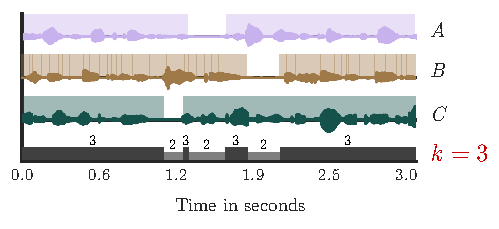
\includegraphics[width=0.8\columnwidth]{Chapters/08_Analysis_CountNet/figures/teaser.pdf}
  \caption{Illustration of three concurrent sources (A, B, C) and their respective activity. Bottom plot shows the mixture (input), the number of concurrently active sources and its maximum \(k\).}%
  \label{fig:teaser}%
\end{figure}

The number of sources is a simple but yet important information to be used in source separation and many other related research fields.
In real world applications, information about the actual number of concurrent speakers is often not available.
\par
The \emph{number of sources} \(k \in \sZ\) appears to be a clearly defined property of a mixture. 
However the meaning of the property can differ, depending on its application.
Let us assume that we have \(L\) sources and mixture of duration \(N\).
Further, I imagine a latent binary \textit{source activity} variable~$v_{nl}\in \left\{ 0,1 \right\}$ that indicates the activity of each source \(l\) and for each time instance \(n\).
Now, concerning the number of sources, two definitions of \(k\) can be imagined:

\begin{description}
\item[A)] maximum number of sources, even if not concurrently active. It is simply the sum of all sources that are active at least once within \(N\). This definition is more useful when the sources can be identified or detected first. This definition can also be considered as ``counting by detection''.
\item[B)] maximum number of concurrent speakers even if the sources belong to the same class. Here, it represents the maximum the mixtures concurrency. This definition is more useful as a preprocessing for a separation system since such a system would only require the number of \texttt{auditory\ streams} and not the number of (non-concurrent) sources. For such approaches it becomes possible to apply separation only when its ``needed''. This definition can also be considered as ``direct count estimation''\footnote{Please note the subtle difference between ``counting'', which refers to a sequential process and ``count estimation'' or ``denumerating'', which directly relate to an integer.}.
\end{description}

At short time scales A) is equal to B) because on such time scale (a few seconds), the sources/instrumentation usually doesn't change. 
In Fig.~\ref{fig:teaser}, I illustrate a setup featuring~$L=3$ unique sources.
At any given time, one can see --- given definition B) --- that at most~$k=L=3$ sources are active at the same time and~$k=2$ could be the outcome if a smaller excerpt would be evaluated.
In this thesis, I will pick definition B when concerned about estimating the number of sources.
However, when dealing with the human ability of estimating the number of sources, such a clear definition can not be made.
For instance, obtaining this number is even more challenging because the definition of a musical source can not clearly be given.
In some scenarios, like popular western music, the sources to be separated, are grouped clear melody, bass, drums and ``other'' (the remainder), in other scenarios, e.g. the ``drums'' would count as multiple instruments.



